\documentclass{beamer}

% Theme choice
\usetheme{CambridgeUS} % professional, clean look
\usecolortheme{default} % colors can be adjusted if desired

% Packages
\usepackage[utf8]{inputenc}
\usepackage{graphicx}   % for including graphics
\usepackage{booktabs}   % for tables
\usepackage{amsmath, amssymb} % for math
\usepackage{hyperref}   % for clickable links

% Title page info
\title[Short Title]{Problem Set 1}
\subtitle{Analysis of Labor Outcomes with PSID}
\author[Your Name]{Tate Mason \\ \smallskip \texttt{Tate.Mason@uga.edu}}
\institute[Your Univ.]{Munro Godfrey Sr. Department of Economics \\ University of Georgia}
\date{\today} % or custom date

% Begin document
\begin{document}

% Title page
\begin{frame}
  \titlepage
\end{frame}

% Outline
\begin{frame}{Outline}
  \tableofcontents
\end{frame}

% Section 1
\section{Introduction}

\begin{frame}{Itinerary}
  \begin{itemize}
    \item Background of PSID
    \item Research Question
    \item Methodology
    \item Results
    \item Conclusion
  \end{itemize}
\end{frame}

\begin{frame}{Background of PSID}
  \begin{itemize}
    \item The PSID is a longitudinal study of household and individual income dynamics 
    \item Grants users an in depth look at long term labor and wealth outcomes 
    \item Maintained by University of Michigan
  \end{itemize}
\end{frame}

\begin{frame}{Research Question}
  \begin{block}{Main Question}
    What are labor and wealth outcomes for men aged 25-60 between 1999-2017?
  \end{block}
  \pause
  \begin{exampleblock}{Subquestions}
    How do these outcomes when stratifying by wealth, educational, and labor 
    characteristics?
  \end{exampleblock}
\end{frame}

% Section 2
\section{Methodology}

\begin{frame}{Data}
  \begin{tabular}{||l|c|c|c|c|c||}
    & 1999 & 2001 & 2003 & 2005 & 2007 & 2009 & 2011 & 2013 & 2015 & 2017 \\
    Sample Size & 81283 &  & & & & & & & & & \\
    Sample by Category: & & & & & & & & \\
    25-30
    31-35
    36-40
    41-45
    46-50
    51-55
    56-60
    Number of Individuals
  \end{tabular}
\end{frame}

\begin{frame}{Age Profile Generation}
  \begin{equation}
    Y_{it} = \gamma\cdot{Age}_{it} + \alpha\cdot{Year}_{it} + \epsilon_{it}
  \end{equation}
  In which $Y_{it}$ is the outcome variable for individual $i$ at time $t$,
  $Age_{it}$ is the age of individual $i$ at time $t$,
  $Year_{it}$ is a set of year fixed effects, and $\epsilon_{it}$ is the error term.
\end{frame}

% Section 3
\section{Results}

\begin{frame}{Main Results - Overall}
  \begin{figure}
    \centering
    \subfloat{
      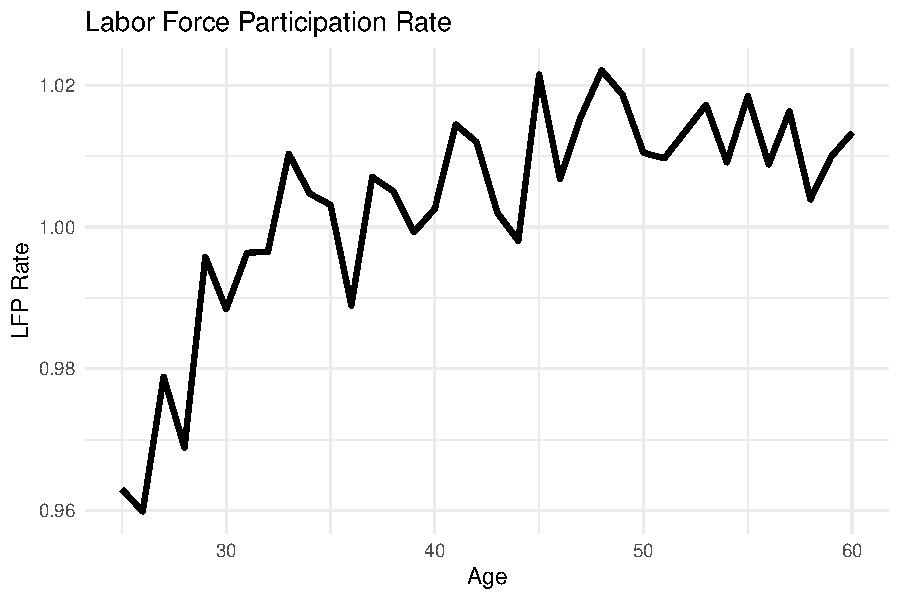
\includegraphics[width=50mm]{~/Schoolwork/Y2S1/Macro/Psets/PS1/output/lfp_age_fe.pdf}
    }
    \subfloat{
      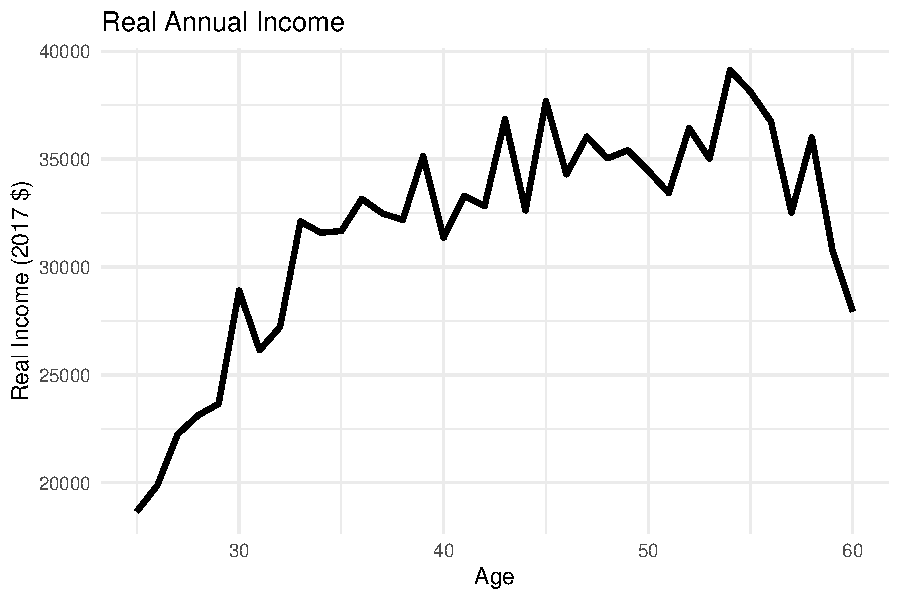
\includegraphics[width=50mm]{~/Schoolwork/Y2S1/Macro/Psets/PS1/output/inc_age_fe.pdf}
    }
  \end{figure}
\end{frame}
\begin{frame}
  \begin{figure}
    \subfloat{
      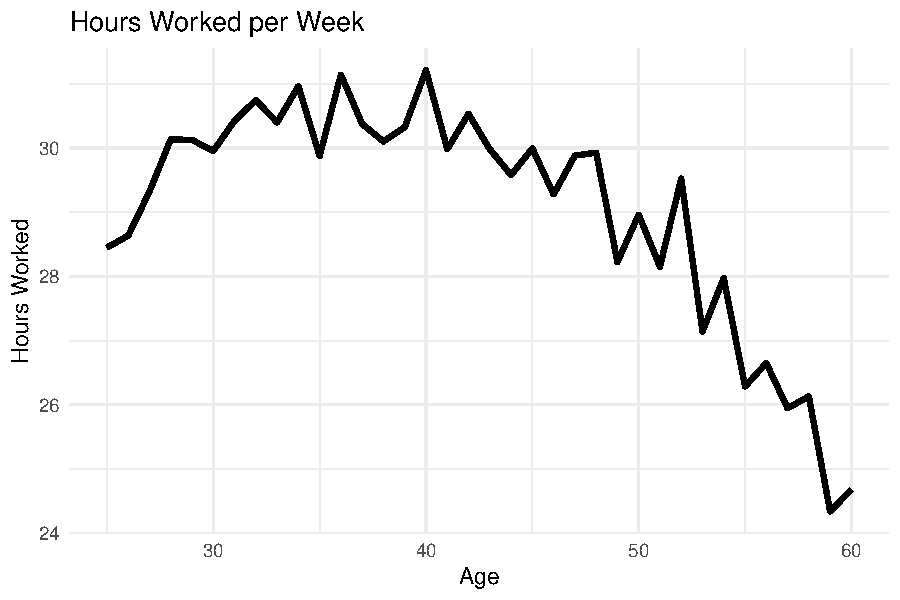
\includegraphics[width=50mm]{~/Schoolwork/Y2S1/Macro/Psets/PS1/output/hr_age_fe.pdf}
    }
    \subfloat{
      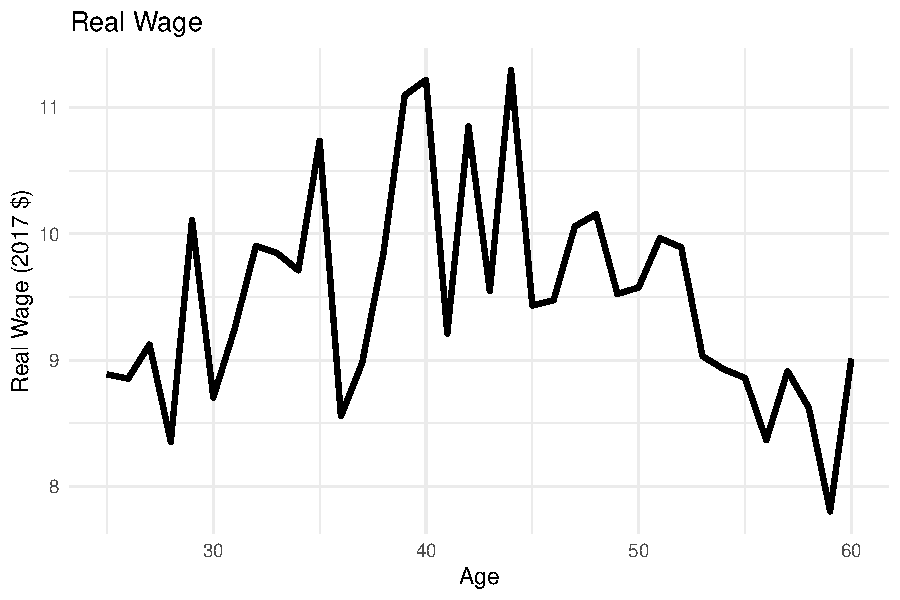
\includegraphics[width=50mm]{~/Schoolwork/Y2S1/Macro/Psets/PS1/output/wage_age_fe.pdf}
    }
  \end{figure}
\end{frame}
\begin{frame}
  \begin{figure}
    \subfloat{
      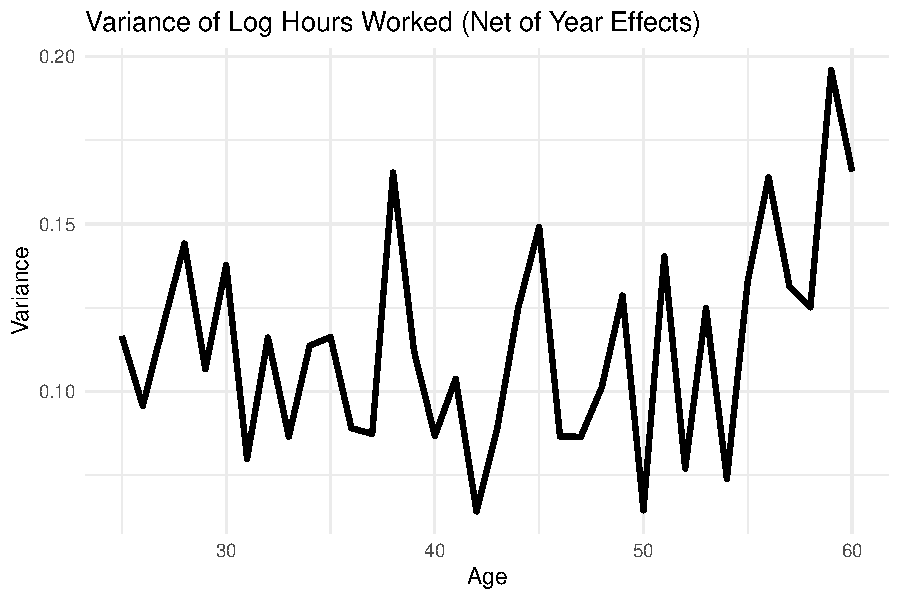
\includegraphics[width=50mm]{~/Schoolwork/Y2S1/Macro/Psets/PS1/output/var_hr_age.pdf}
    }
    \subfloat{
      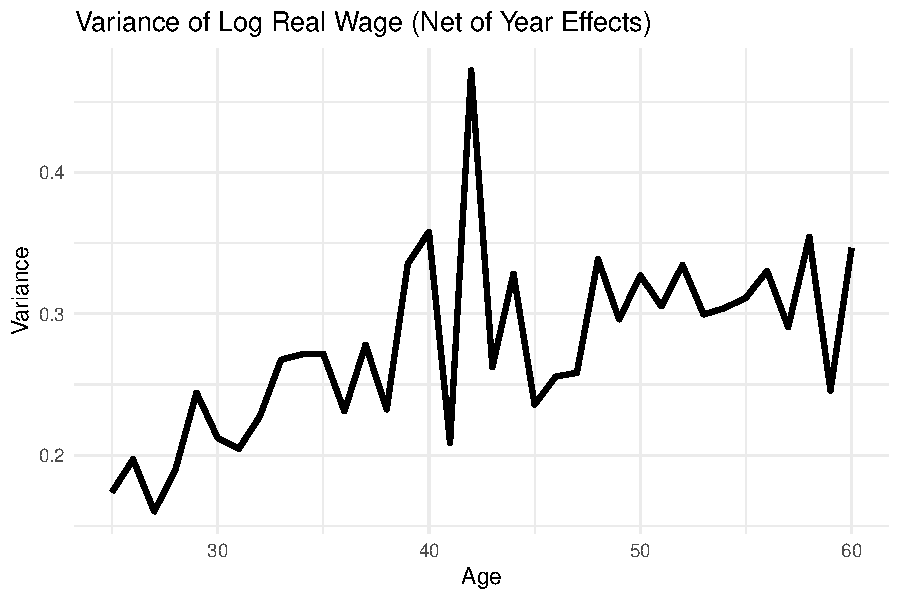
\includegraphics[width=50mm]{~/Schoolwork/Y2S1/Macro/Psets/PS1/output/var_wage_age.pdf}
    }
  \end{figure}
\end{frame}

\begin{frame}{Results - Stratified by Education}
  \begin{figure}
    \centering
    \subfloat{
      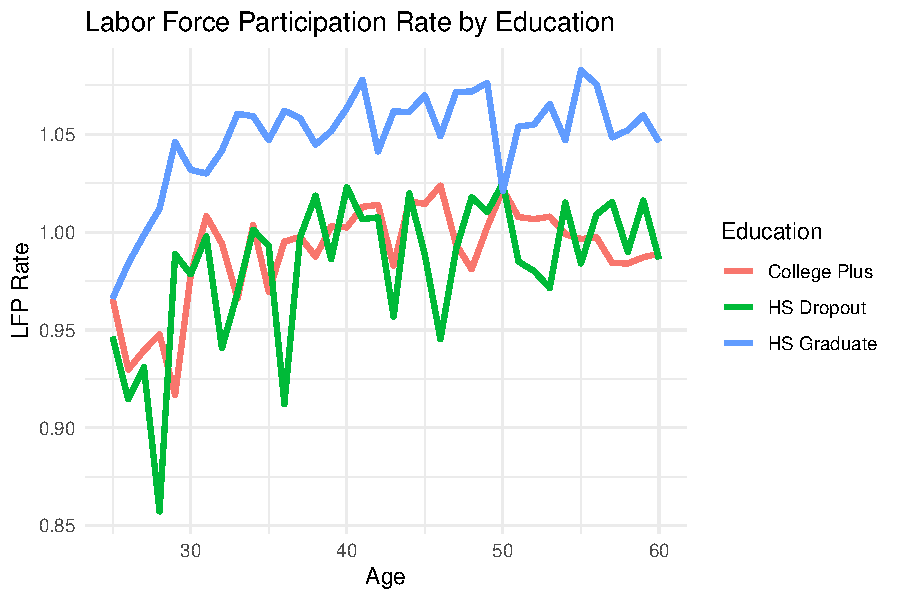
\includegraphics[width=50mm]{~/Schoolwork/Y2S1/Macro/Psets/PS1/output/lfp_age_fe_educ.pdf}
    }
    \subfloat{
      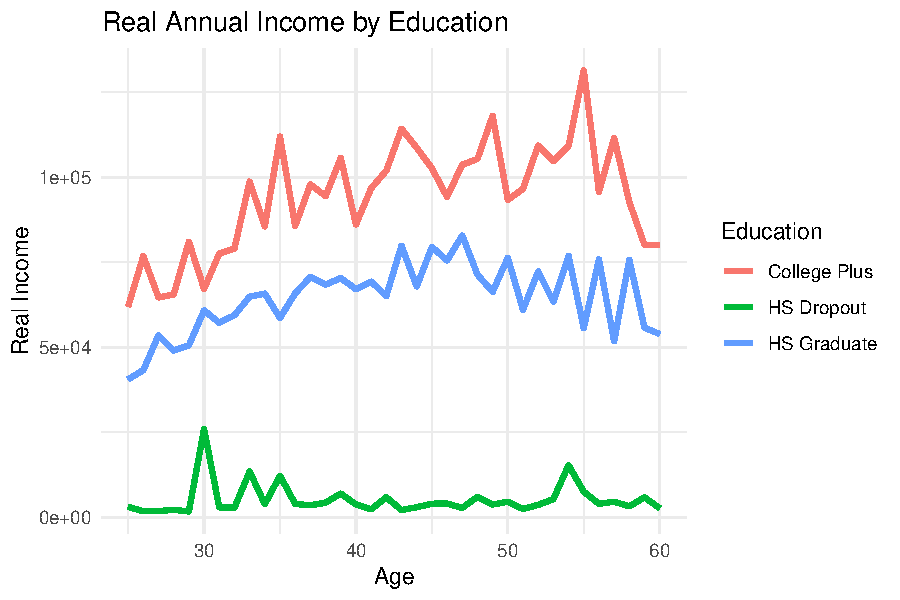
\includegraphics[width=50mm]{~/Schoolwork/Y2S1/Macro/Psets/PS1/output/inc_age_fe_educ.pdf}
    }
  \end{figure}
\end{frame}

\begin{frame}
  \begin{figure}
    \subfloat{
      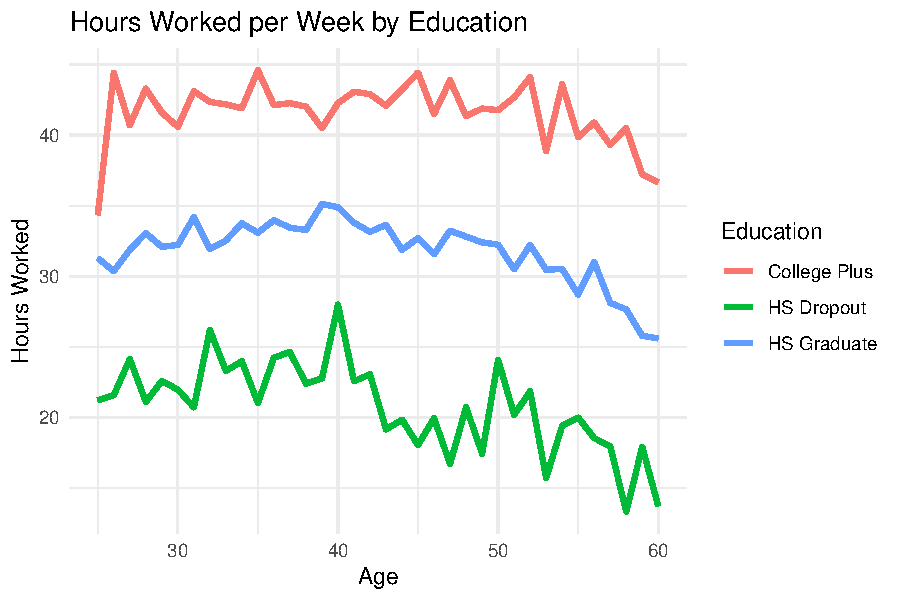
\includegraphics[width=50mm]{~/Schoolwork/Y2S1/Macro/Psets/PS1/output/hr_age_fe_educ.pdf}
    }
    \subfloat{
      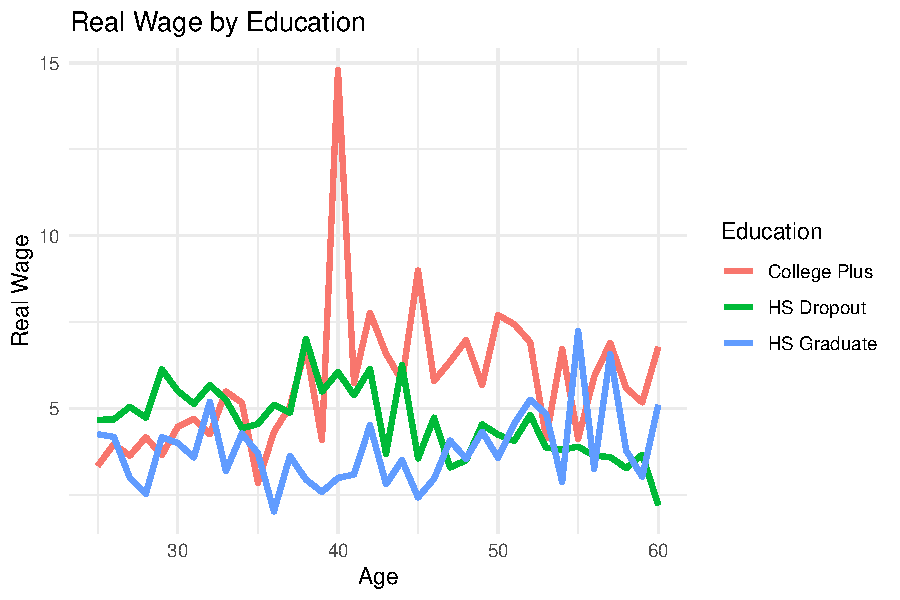
\includegraphics[width=50mm]{~/Schoolwork/Y2S1/Macro/Psets/PS1/output/wage_age_fe_educ.pdf}
    }
  \end{figure}
\end{frame}

\begin{frame}
  \begin{figure}
    \subfloat{
      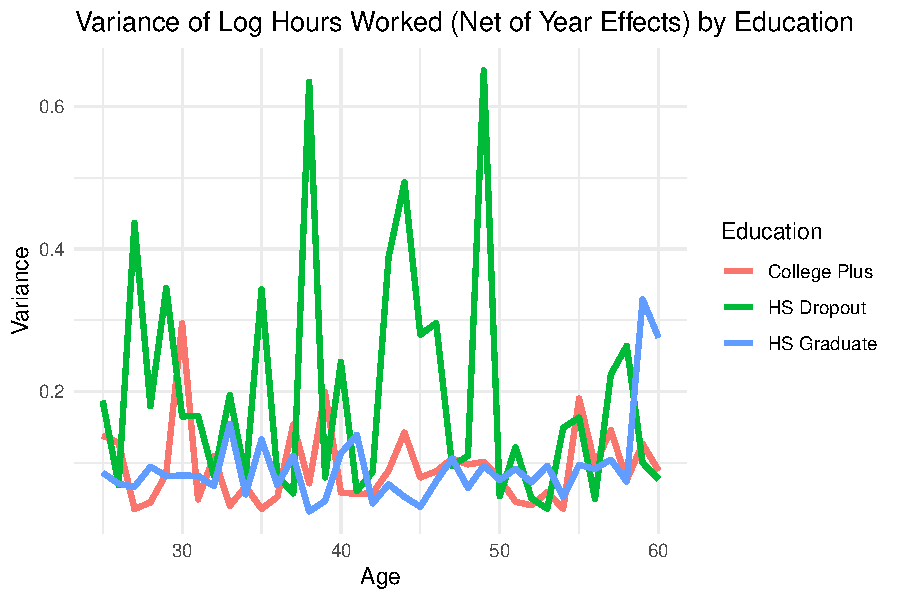
\includegraphics[width=50mm]{~/Schoolwork/Y2S1/Macro/Psets/PS1/output/var_hr_age_educ.pdf}
    }
    \subfloat{
      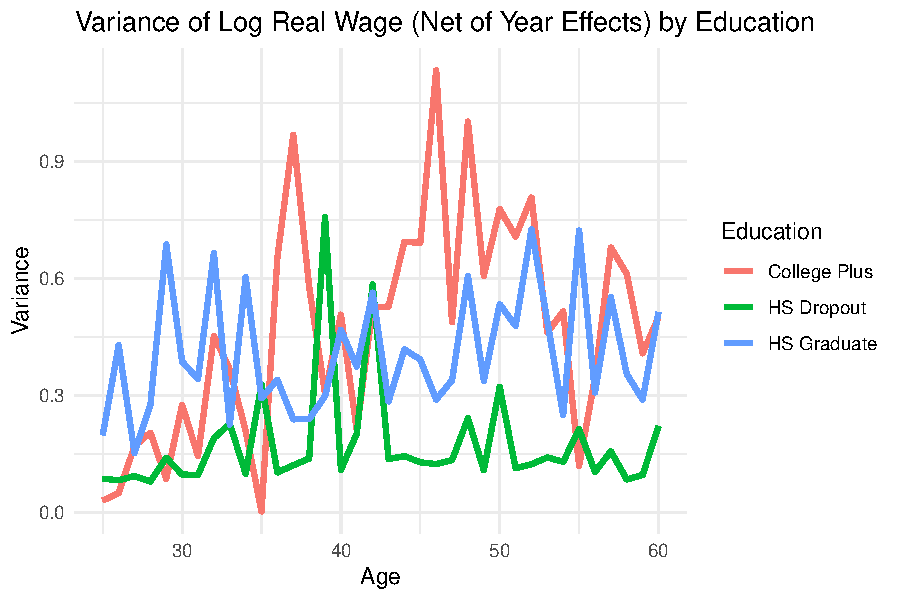
\includegraphics[width=50mm]{~/Schoolwork/Y2S1/Macro/Psets/PS1/output/var_wage_age_educ.pdf}
    }
  \end{figure}
\end{frame}

\begin{frame}{Results - Stratified by Industry}
  \begin{figure}
    \centering
    \subfloat{
      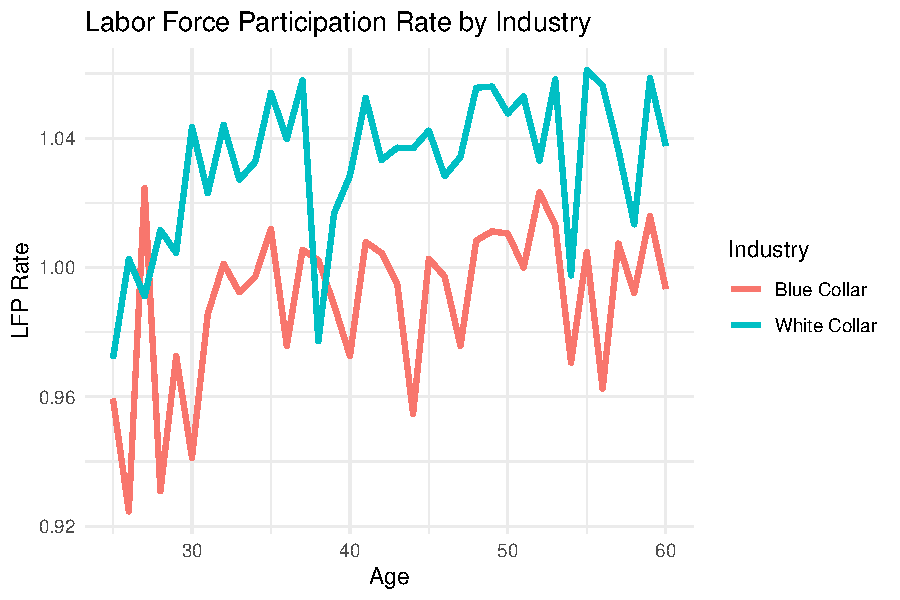
\includegraphics[width=50mm]{~/Schoolwork/Y2S1/Macro/Psets/PS1/output/lfp_age_fe_ind.pdf}
    }
    \subfloat{
      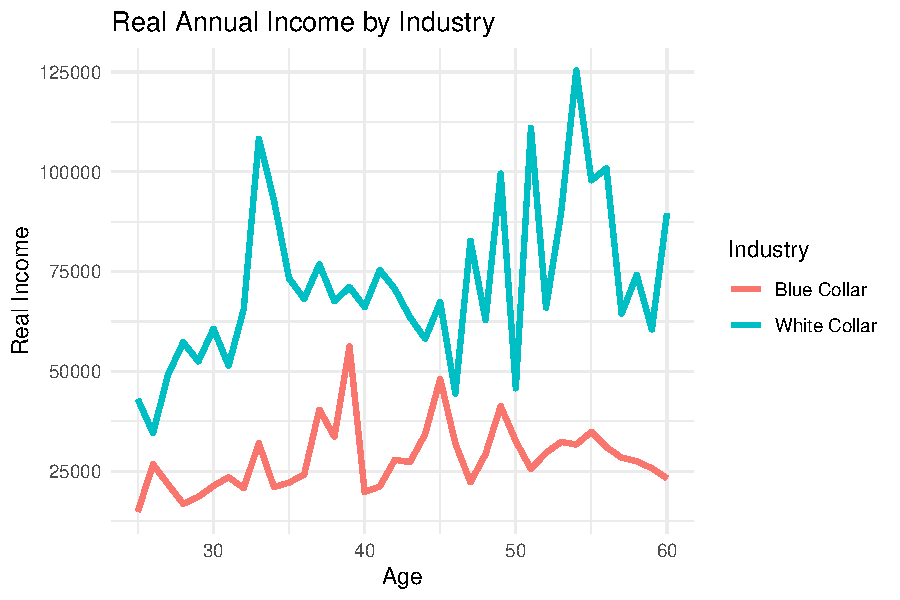
\includegraphics[width=50mm]{~/Schoolwork/Y2S1/Macro/Psets/PS1/output/inc_age_fe_ind.pdf}
    }
  \end{figure}
\end{frame}
\begin{frame}
  \begin{figure}
    \subfloat{
      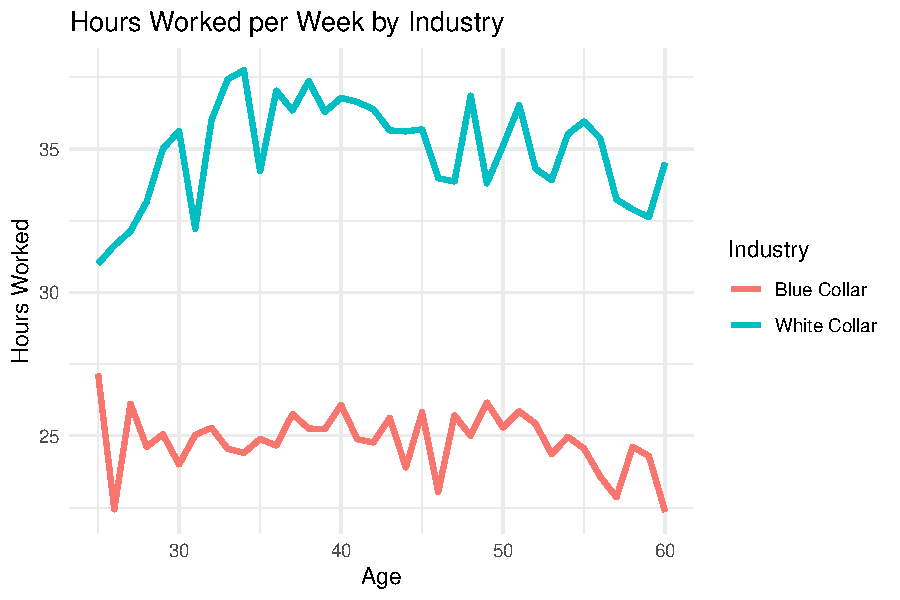
\includegraphics[width=50mm]{~/Schoolwork/Y2S1/Macro/Psets/PS1/output/hr_age_fe_ind.pdf}
    }
    \subfloat{
      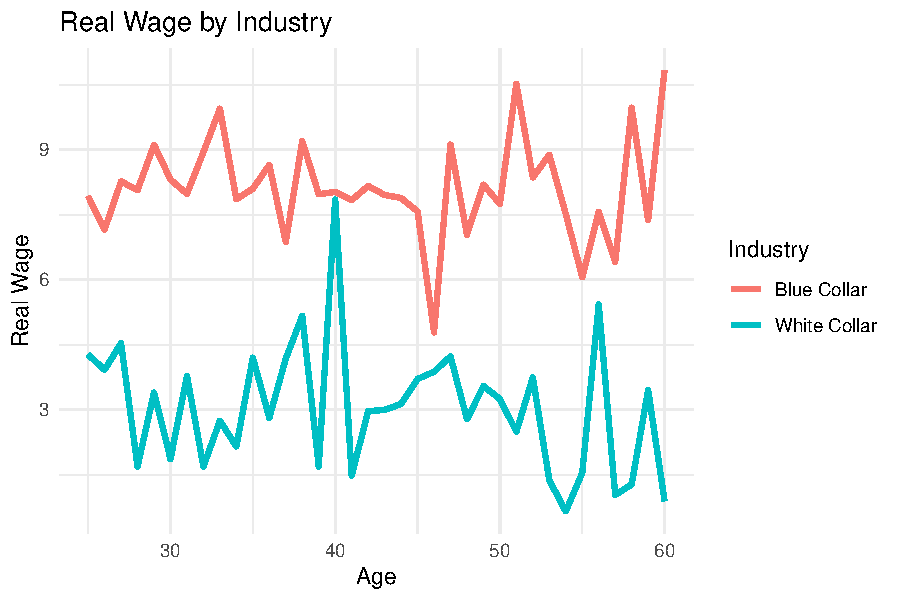
\includegraphics[width=50mm]{~/Schoolwork/Y2S1/Macro/Psets/PS1/output/wage_age_fe_ind.pdf}
    }
  \end{figure}
\end{frame}

\begin{frame}
  \begin{figure}
    \subfloat{
      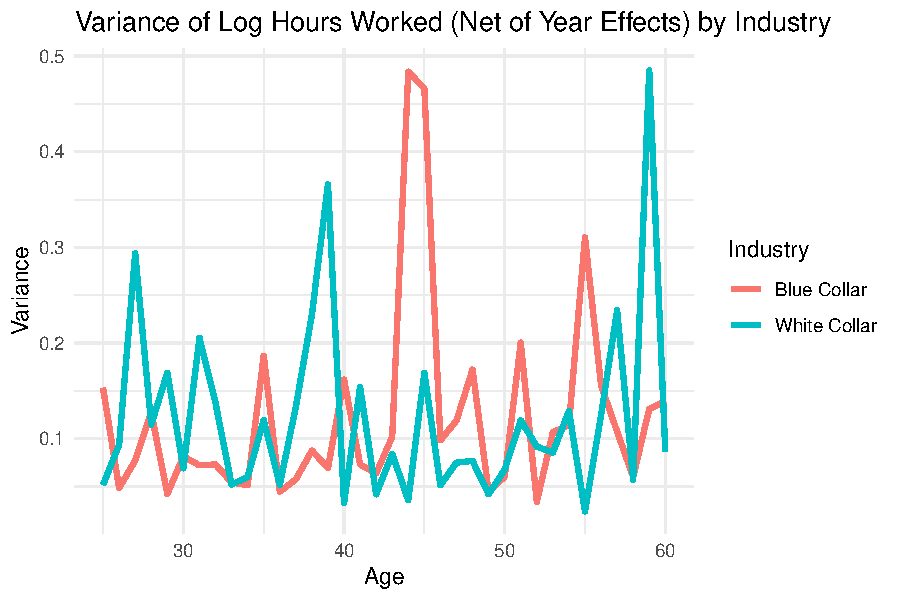
\includegraphics[width=50mm]{~/Schoolwork/Y2S1/Macro/Psets/PS1/output/var_hr_age_ind.pdf}
    }
    \subfloat{
      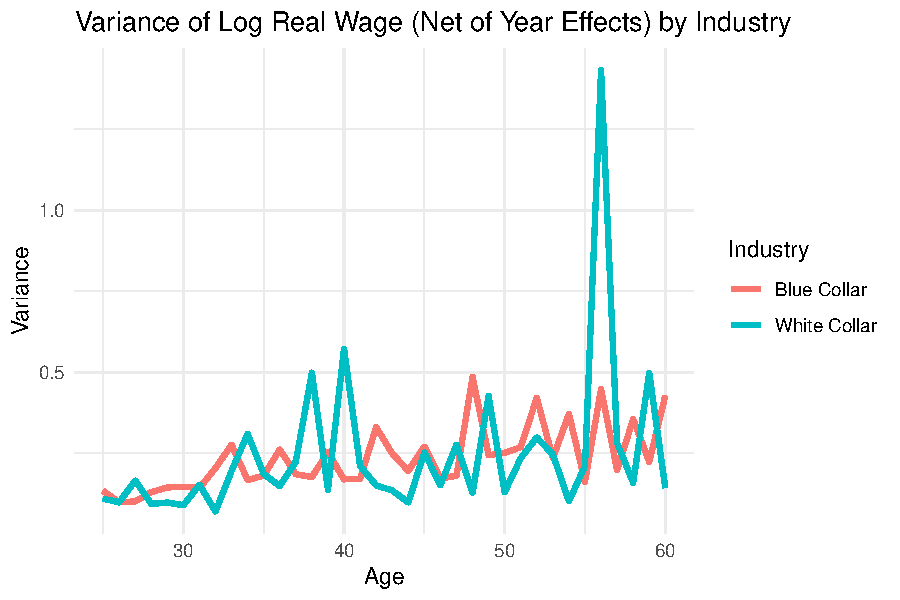
\includegraphics[width=50mm]{~/Schoolwork/Y2S1/Macro/Psets/PS1/output/var_wage_age_ind.pdf}
    } 
  \end{figure}
\end{frame}

\begin{frame}{Results - Stratified by Wealth}
  \begin{figure}
    \centering
    \subfloat{
      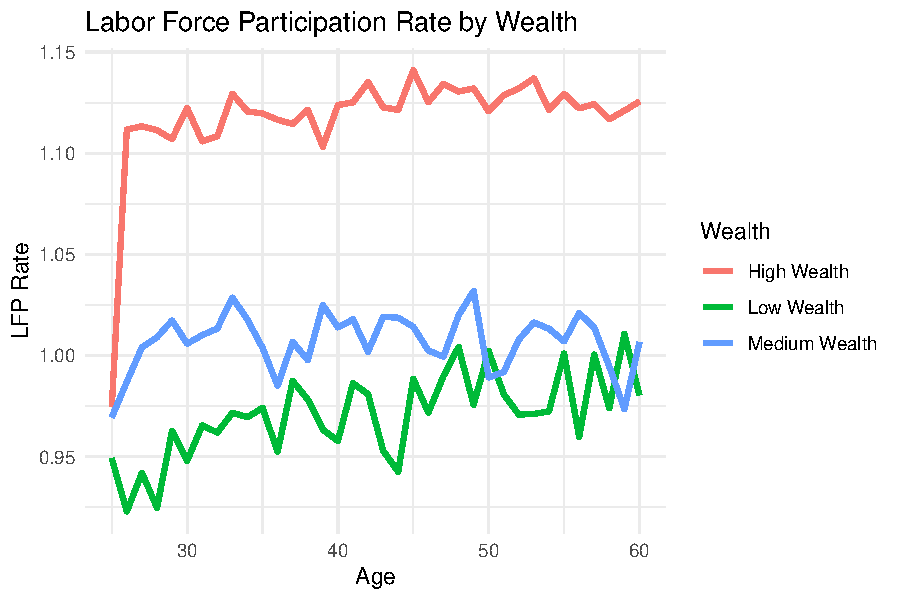
\includegraphics[width=50mm]{~/Schoolwork/Y2S1/Macro/Psets/PS1/output/lfp_age_fe_wealth.pdf}
    }
    \subfloat{
      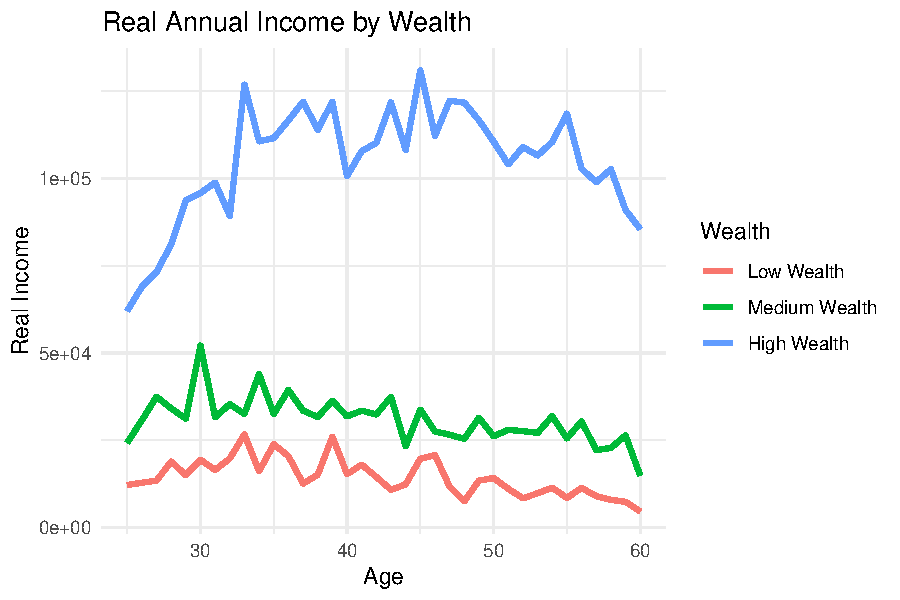
\includegraphics[width=50mm]{~/Schoolwork/Y2S1/Macro/Psets/PS1/output/inc_age_fe_wealth.pdf}
    }
  \end{figure}
\end{frame}
\begin{frame}
  \begin{figure}
    \subfloat{
      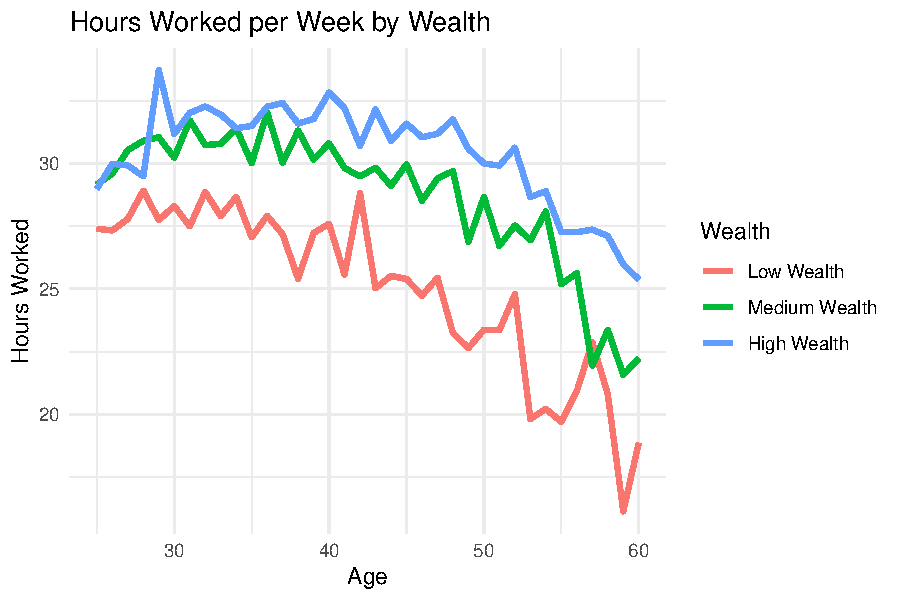
\includegraphics[width=50mm]{~/Schoolwork/Y2S1/Macro/Psets/PS1/output/hr_age_fe_wealth.pdf}
    }
    \subfloat{
      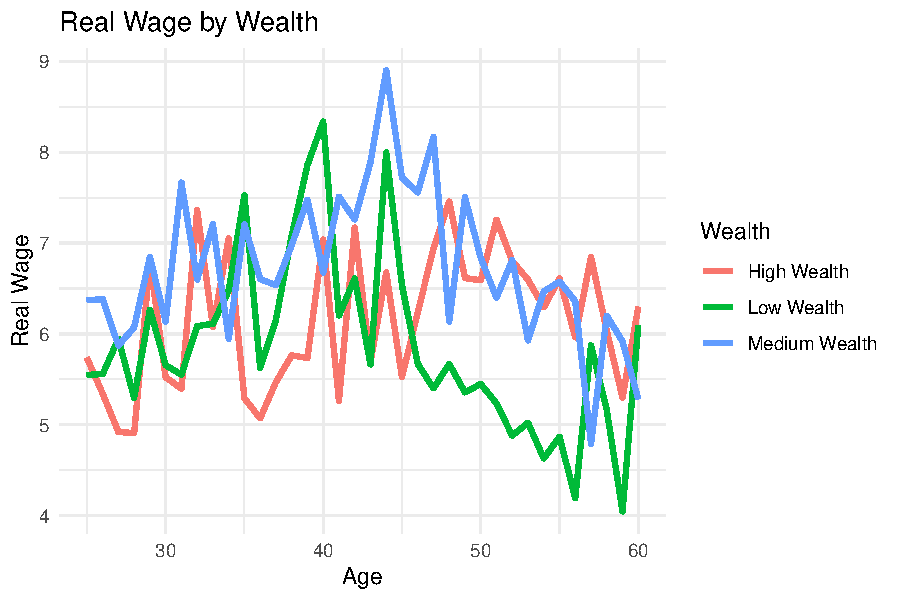
\includegraphics[width=50mm]{~/Schoolwork/Y2S1/Macro/Psets/PS1/output/wage_age_fe_wealth.pdf}
    }
  \end{figure}
\end{frame}
\begin{frame}
  \begin{figure}
    \subfloat{
      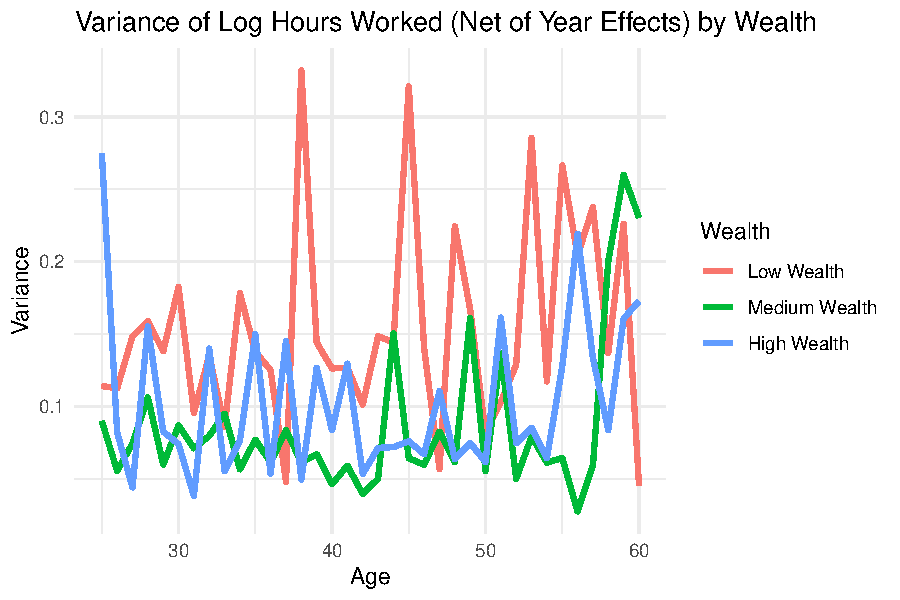
\includegraphics[width=50mm]{~/Schoolwork/Y2S1/Macro/Psets/PS1/output/var_hr_age_wealth.pdf}
    }
    \subfloat{
      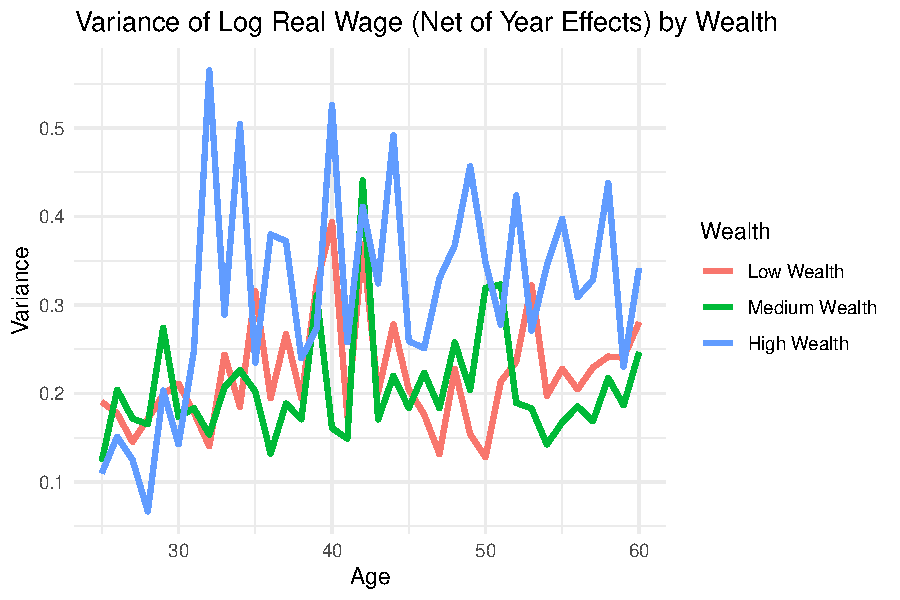
\includegraphics[width=50mm]{~/Schoolwork/Y2S1/Macro/Psets/PS1/output/var_wage_age_wealth.pdf}
    }
  \end{figure}
\end{frame}
% Section 4
\section{Conclusion}

\begin{frame}{Conclusion}
  \begin{itemize}
    \item We see much of what we would expect in the data 
    \item Hourly wage is not what I would expect 
    \item Variance is massive, especially in wages 
  \end{itemize}
\end{frame}

\end{document}
